\section{Ejercicio 2}
\subsection{Introducción}
En esta sección desarrollaremos el diseño de una máquina de estados de Mealy capaz de reconocer la secuencia 1-1-0-1, enviada de forma serial y una vez reconocida la secuencia, obtendremos una salida de encendido. Mientras que, en el caso contrario tendremos una salida apagada.\\
La misma consiste en 4 estados, un default que va a ser el estado donde siempre va a volver en caso de error y 3 estados de transición. El estado default va a ser el estado inicial de la misma.\\
A continuación podemos observar el diagrama de la misma:\\
\begin{figure}[H]
	\centering
	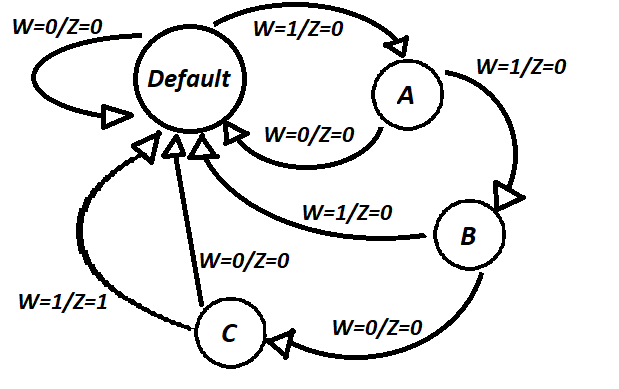
\includegraphics[scale=0.35]{Ejercicio2/Diagrama_de_estados.png}
	\caption{Diagrama de estados}
	\label{f:Mealy}
\end{figure}
En donde Z es la salida, W es la entrada y las flechas indican hacia donde se realiza la transición así como bajo qué valor de la entrada sucede la misma.\\
De la figura \ref{f:Mealy} podemos obtener la siguiente tabla de estados:\\
\begin{table}[h!]
	\begin{center}
		\caption{Tabla de estados}
		\begin{tabular}{|c|c c|c c|}
		\hline
		\multirow{2}{*}{Estado Actual} & \multicolumn{2}{|c|}{Estado siguiente} & \multicolumn{2}{|c|}{Salida}\\
		& $W=0$ & $W=1$ & $W=0$ & $W=1$\\
		\hline
		Default & Default & A & 0 & 0\\
		\hline
		A & Default & B & 0 & 0\\
		\hline
		B & C & Default & 0 & 0\\
		\hline
		C & Default & Default & 0 & 0\\
		\hline
		\end{tabular}
	\end{center}
\end{table}\\
\subsection{Implementación}
Para implementar una máquina de Mealy utilizamos el siguiente circuito secuencial genérico:\\
\begin{figure}[H]
	\centering
	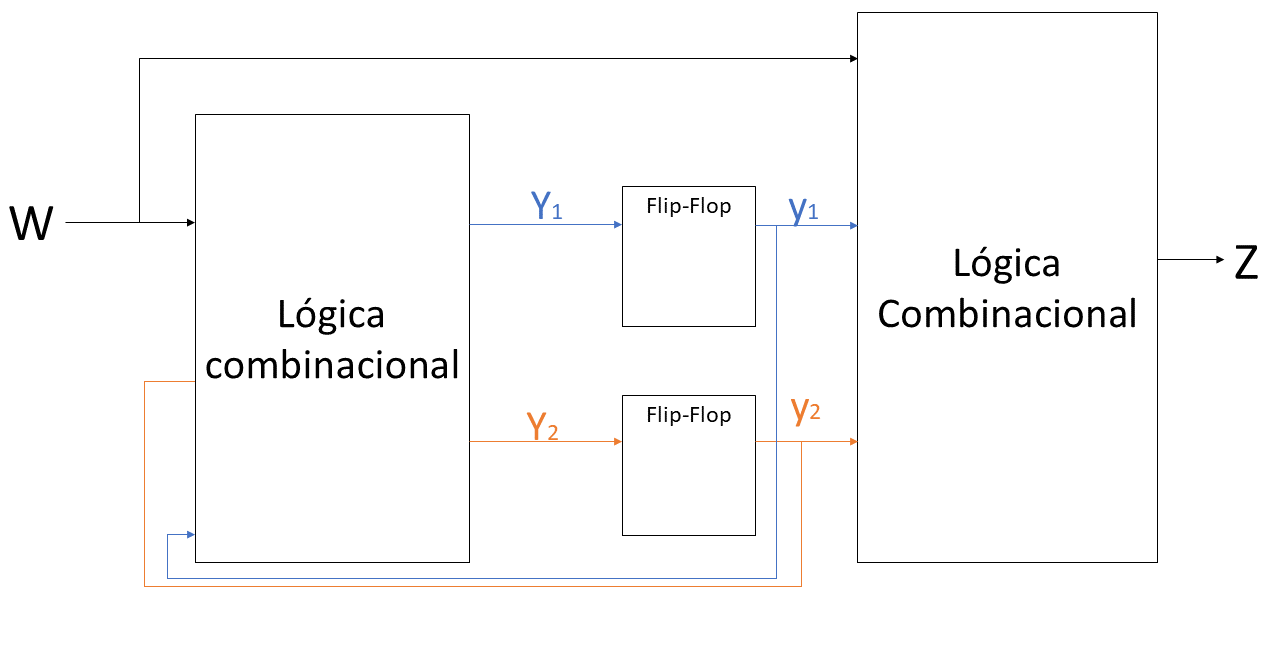
\includegraphics[scale=0.3]{Ejercicio2/Maquina_Mealy.png}
	\caption{Circuito genérico}
\end{figure}
\subsubsection{Asignación de estados}
Por último, se realiza la asignación de los estados dando lugar a la siguiente tabla:\\
%Tabla de asignacion
\begin{table}[H]
	\begin{center}
		\caption{Tabla de estados asignados}
		\label{t:talba}
		\begin{tabular}{|c|c|c c|c c|}
		\hline
		\multirow{3}{*}{Estado Actual} & {Asignado del estado actual} & \multicolumn{2}{|c|}{Estado siguiente} & \multicolumn{2}{|c|}{Salida}\\
		& \multirow{2}{*}{$y_2y_1$} & $W=0$ & $W=1$ & \multirow{3}{*}{$W=0$} & \multirow{3}{*}{$W=1$}\\
		& & $Y_2Y_1$ & $Y_2Y_1$ & &\\
		\hline
		Default & 00 & 00 & 01 & 0 & 0\\
		\hline
		A & 01 & 00 & 10 & 0 & 0\\
		\hline
		B & 10 & 11 & 00 & 0 & 0\\
		\hline
		C & 11 & 00 & 00 & 0 & 1\\
		\hline
		\end{tabular}
	\end{center}
\end{table}
\subsubsection{Mapas de Karnaugh}
A partir de la tabla \ref{t:talba} se obtienen los siguientes mapas de Karnaugh:\\
%Mapas de Karnaugh 
\begin{center}
	\hspace*{\fill}
	\begin{tikzpicture}[x=8mm,y=8mm]
    	\K[x bits = 2, y bits = 1, label={$Y_1$},
       	variable names = {$y_2$,$y_1$,$W$,}]
    	{ 
      	000,0,    
      	001,1,   
      	010,0,   
      	011,0,       
      	100,1, 
      	101,0,
      	110,0,
 	  	111,0,
    	}
    	\newcommand*{\myKG}[4][0.1]{\KG[x bits = 2,y bits = 1,group opacity = #1,
        	          #2]{#3}{#4}}
    	\myKG     {group color = green,  group distance=0.35}{001}{001}
		\myKG     {group color = green,  group distance=0.35}{100}{100}
    	%=====================================================================
    	% in picture comments
    	%=====================================================================	
    	\path (1,-1.5) node[anchor = north, align = left] (eq1){%
    	$Y_1 = 
       	\ul{green}{$\ol{y_1}\,\ol{y_2}\,{W}+\ol{y_1}\,{y_2}\,\ol{W}\,$} 
    	$};
	\end{tikzpicture}
	\hspace{2mm}
	\begin{tikzpicture}[x=8mm,y=8mm]
    	\K[x bits = 2, y bits = 1, label={$Y_2$},
       	variable names = {$y_2$,$y_1$,$W$,}]
    	{ 
      	000,0,    
      	001,0,   
      	010,0,   
      	011,1,       
      	100,1, 
      	101,0,
      	110,0,
 	  	111,0,
    	}
    	\newcommand*{\myKG}[4][0.1]{\KG[x bits = 2,y bits = 1,group opacity = #1,
        	          #2]{#3}{#4}}
    	\myKG     {group color = green,  group distance=0.35}{011}{011}
		\myKG     {group color = green,  group distance=0.35}{100}{100}
    	%=====================================================================
    	% in picture comments
    	%=====================================================================
    	\path (1,-1.5) node[anchor = north, align = left] (eq1){%
    	$Y_2 = 
       	\ul{green}{$\ol{y_1}\,{y_2}\,\ol{W}+{y_1}\,\ol{y_2}\,{W}\,$} 
    	$};
	\end{tikzpicture}
	\hspace{2mm}
	\begin{tikzpicture}[x=8mm,y=8mm]
    	\K[x bits = 2, y bits = 1, label={$Z$},
       	variable names = {$y_2$,$y_1$,$W$,}]
    	{ 
      	000,0,    
      	001,0,   
      	010,0,   
      	011,0,       
      	100,0, 
      	101,0,
      	110,0,
 	  	111,1,
    	}
    	\newcommand*{\myKG}[4][0.1]{\KG[x bits = 2,y bits = 1,group opacity = #1,
        	          #2]{#3}{#4}}
    	\myKG     {group color = green,  group distance=0.35}{111}{111}
    	%=====================================================================
    	% in picture comments
    	%=====================================================================	
    	\path (1,-1.5) node[anchor = north, align = left] (eq1){%
    	$Z = 
       	\ul{green}{${y_1}\,{y_2}\,{W}$} 
    	$};
	\end{tikzpicture}
	\hspace*{\fill}
\end{center}
\subsubsection{Circuito resultante}
Para la realización del circuito utilizamos los Flip-Flop D debido a que poseen una relación directa con las variables de estado $y_i$ y $Y_i$. Donde las variables $y_i=Q_i$, pero cabe mencionar que esto es equivalente para todos los distintos tipos de Flip-Flop y $Y_i=D_i$ que es exclusivo del mismo.
Finalmente, a partir de los mapas de Karnaugh anteriormente mostrados, surge el siguiente circuito:\\
\begin{figure}[H]
	\centering
	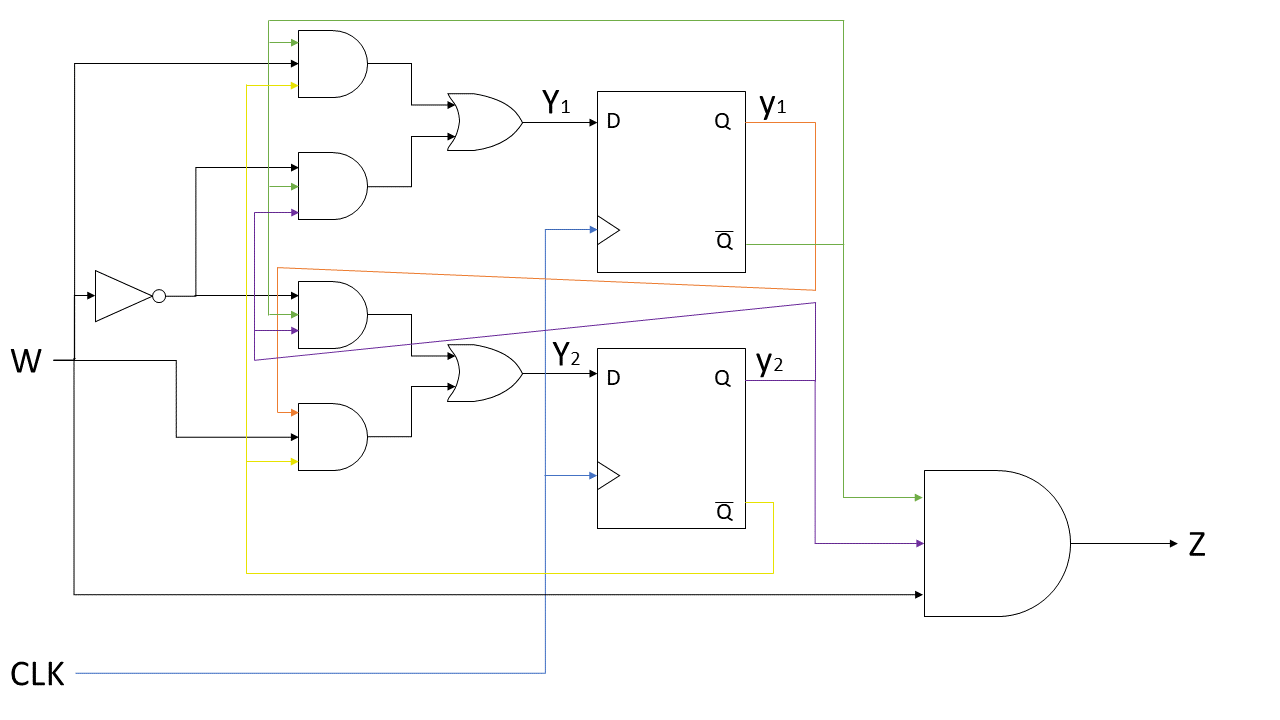
\includegraphics[scale=0.4]{Ejercicio2/Circuito.png}
	\caption{Circuito genérico}
\end{figure}
\subsection{Simulación}
Luego, se generó la correspondiente simulación en Verilog, el cual nos brinda el comportamiento ideal del mismo. Esto dio lugar al siguiente resultado:\\
\begin{figure}[H]
	\centering
	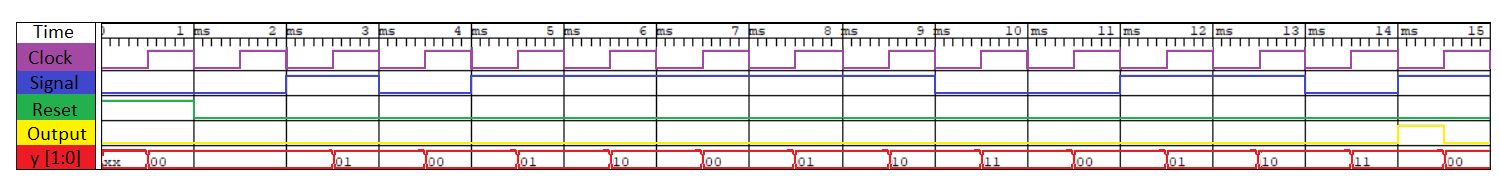
\includegraphics[scale=0.5]{Ejercicio2/Simulacion.png}
	\caption{Circuito genérico}
\end{figure}